\documentclass[xcolor={table}]{beamer}
\usepackage[english]{babel}
\usepackage[utf8]{inputenc}

\usepackage{hyperref}
\usepackage{url}
\usepackage{amsmath}
\usepackage{graphicx}
\usepackage{animate}
\usepackage{subcaption}
\usepackage{multicol}
\usepackage[full, italic, slant]{complexity}
\usepackage{appendixnumberbeamer}


\expandafter\def\expandafter\insertshorttitle\expandafter{%
  \insertshorttitle\hfill\insertframenumber\,/\,\inserttotalframenumber}

\def\*{{\bf FIXME: }}

\setbeamertemplate{caption}[numbered]
\setbeamertemplate{bibliography item}{\insertbiblabel}
\newtheorem{deff}{Definícia}[section]

\mode<presentation> {
    \usetheme{Warsaw}
    \usecolortheme{seahorse}
    \usecolortheme{rose}
    \usefonttheme{professionalfonts}
    \setbeamercovered{transparent}
}

\definecolor{bloodred}{RGB}{200,0,0}


\title{Flowing gradient through SVD}
\author{Bc. Vladimír Macko}
\institute{RNDr. Radim Řehůřek, Ph.D}

\begin{document}
        
\begin{frame}
    \titlepage
\end{frame}
    
\begin{frame}{Overview}
    \begin{block}{}
        \begin{itemize}
            \item Introduction to the problematics
            \item Problem outline
            \item Our work
            \item Results
            \item Plans
        \end{itemize}
    \end{block}
\end{frame}


\section{Introduction}
\begin{frame}{Document classification}
	\begin{block}{}
		\emph{This was a terrible movie}
	\end{block}
	
    \begin{block}{}   
        \begin{itemize}
            \item create representation for words
            \item create representation for document
            \item predict
        \end{itemize}
    \end{block}
\end{frame} 

\begin{frame}{Word vectors}
    \begin{columns}
       \column{0.5\linewidth}
        Local representation
        \begin{block}{}
            One hot encoding
        \end{block}

        \column{0.5\linewidth}
        Distributed representation
        \begin{block}{Count based}
            Factorization of co-occurrence matrix
            
            LSA (SVD)
        \end{block}
        \begin{block}{Prediction based}
            Trained neural network

            Skip gram    
        \end{block}    
   \end{columns}
\end{frame} 

\begin{frame}{Count vs. prediction}
    \begin{block}{Prediction}
        \begin{itemize}
            \item extremely popular
            \item huge performance gains
            \item less memory demanding
        \end{itemize}
    \end{block}

    \begin{block}{Count}
        \begin{itemize}
            \item less hyperparameters
            \item easier to ``train''
            \item teoreticaly based
        \end{itemize}
    \end{block}
\end{frame} 

\begin{frame}{Count vs prediction}
    \begin{block}{Glove vectors as explicit factorization}
        \begin{itemize}
            \item Neural word embedding as implicit matrix factorization \cite{levy2014neural}
        \end{itemize}
    \end{block}

    \begin{block}{Hyperparameters matter}
        \begin{itemize}
            \item Improving distributional similarity with lessons learned from word embeddings \cite{levy2015improving}
        \end{itemize}
    \end{block}

    \begin{block}{Does not work well on small datasets}
        \begin{itemize}
            \item Comparative study of LSA vs Word2vec embeddings in small corpora \cite{altszyler2016comparative}
        \end{itemize}
    \end{block}
\end{frame} 


\section{Problem outline}
\begin{frame}{LSA problems}
    \begin{block}{}
        \begin{itemize}
            \item Sensitive to preprocessing
            \item Sensitive to weights
            \item Unsupervised and can forget things
        \end{itemize}
    \end{block}
\end{frame} 

\begin{frame}{Current solutions}
    \begin{block}{}
        \begin{itemize}
            \item Preprocessing
            \item Weight - Mutual information \cite{wu2017balancing}, \cite{deng2014study}
            \item Supervised weights: TF-KLD \cite{ji2013discriminative}, \cite{lan2009supervised}
        \end{itemize}
    \end{block}
\end{frame} 

\section{Our work}
\begin{frame}{Our system}
    \begin{block}{Baseline}
        Co-occurrence matrix, rescale weight, factorization, prediction
        
        Training the predictor
    \end{block}

    \begin{block}{Our}
        Co-occurrence matrix, rescale weight, factorization, prediction

        Compute gradient with respect to the weights
    \end{block}
    
    LSA used in similar manner in \cite{ionescu2015training}
\end{frame} 

\begin{frame}{Gradient descent}
	\begin{columns}	
	\column{0.5\linewidth}
	\begin{itemize}
        \item Co-occurrence matrix $M$
        \item Weight vector $t$
	\end{itemize}
	\column{0.5\linewidth}
	\begin{itemize}
        \item SVD: $U \Sigma V^T$
        \item Simple classifier: $\sigma (x \theta + b)$
	\end{itemize}	
	\end{columns}

	\begin{block}{}
	\begin{itemize}
        \item Reweighted matrix $M \circ t$
        \item SVD decomposition $U \Sigma V^T$
        \item Compute embedding $x = d \circ t U$
        \item Train classifier $\hat{y} = \sigma (x \theta + b)$
        \item Compute error $E = \frac{1}{2}(\hat{y}-y)^2$
        \item Compute derivation $\frac{\partial E}{\partial t} = (\hat{y} -y) \sigma{\hat{y}} (1-\sigma{\hat{y}})\Theta U$
        \item Update weights: $t = t - \alpha \frac{\partial E}{\partial t}$
	\end{itemize}	
	\end{block}
\end{frame} 

\begin{frame}{Evaluation}
    \begin{block}{Datasets from SentEval \cite{conneau2017supervised}}
        \begin{itemize}
	        \item Costumer review dataset
	        \item Movie review
	        \item Subjective vs objective
	        \item Opinion polarity	        
        \end{itemize}
    \end{block}
    
    
\end{frame} 

\section{Results}
\begin{frame}{}
	\begin{columns}
		\column{0.5\linewidth}
   				\begin{figure}[H]
        			\centering
        			\caption*{SVD + logistic regression}
        			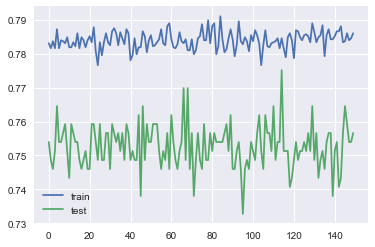
\includegraphics[height=0.4\textheight]{images/CRDataset.png}
        			\caption{Precision of baseline on CR dataset for multiple tries}
        		\end{figure}
        	\column{0.5\linewidth}

        		\begin{figure}[H]
        			\centering
        			\caption*{TFIDF + SVD + logistic regression}
        			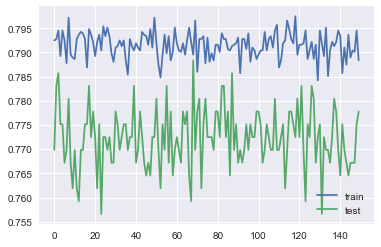
\includegraphics[height=0.4\textheight]{images/CRDataset_tfidf.png}
        			\caption{Precision of baseline on CR dataset for multiple tries}
        		\end{figure}
	\end{columns}
        		
\end{frame} 

\begin{frame}{}
	\begin{columns}
		\column{0.5\linewidth}
   				\begin{figure}[H]
        			\centering
        			\caption*{SVD + LR + gradient}
        			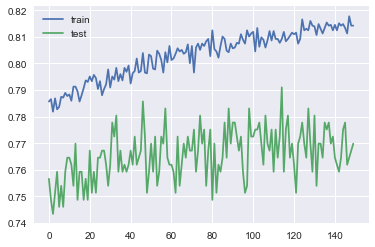
\includegraphics[height=0.4\textheight]{images/CRDataset_grad.png}
        			\caption{Precision of weight improving on CR dataset for multiple epochs}
        		\end{figure}
        	\column{0.5\linewidth}

        		\begin{figure}[H]
        			\centering
        			\caption*{TFIDF + SVD + LR + gradient}
        			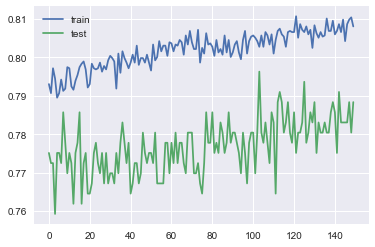
\includegraphics[height=0.4\textheight]{images/CRDataset_tfidf_grad.png}
        			\caption{Precision of tfidf weight improving on CR dataset for multiple epochs}
        		\end{figure}
	\end{columns}        		
\end{frame} 

\begin{frame}{}
	\begin{columns}
		\column{0.5\linewidth}
   				\begin{figure}[H]
        			\centering
        			\caption*{SVD + LR + gradient}
        			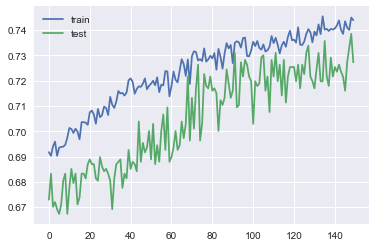
\includegraphics[height=0.4\textheight]{images/MRDataset_grad.png}
        			\caption{Precision of weight improving on MR dataset for multiple epochs}
        		\end{figure}
        	\column{0.5\linewidth}

        		\begin{figure}[H]
        			\centering
        			\caption*{TFIDF + SVD + LR + gradient}
        			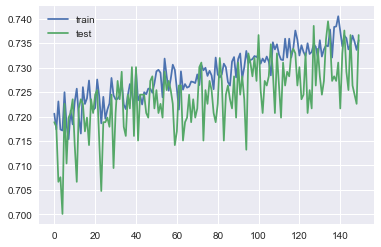
\includegraphics[height=0.4\textheight]{images/MRDataset_tfidf_grad.png}
        			\caption{Precision of tfidf weight improving on MR dataset for multiple epochs}
        		\end{figure}
	\end{columns}        		
\end{frame} 

\begin{frame}{}
	\begin{columns}
		\column{0.5\linewidth}
   				\begin{figure}[H]
        			\centering
        			\caption*{SVD + LR + gradient}
        			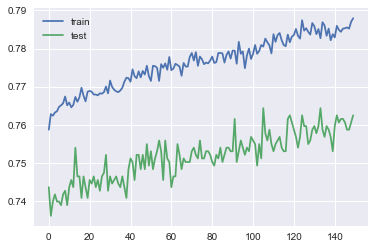
\includegraphics[height=0.4\textheight]{images/MPQADataset_grad.png}
        			\caption{Precision of weight improving on MPQA dataset for multiple epochs}
        		\end{figure}
        	\column{0.5\linewidth}

        		\begin{figure}[H]
        			\centering
        			\caption*{TFIDF + SVD + LR + gradient}
        			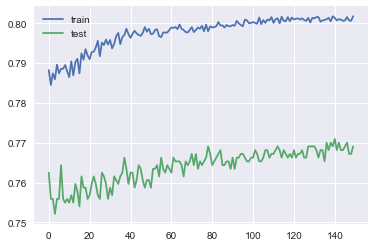
\includegraphics[height=0.4\textheight]{images/MPQADataset_tfidf_grad.png}
        			\caption{Precision of tfidf weight improving on MPQA dataset for multiple epochs}
        		\end{figure}
	\end{columns}        		
\end{frame} 

\begin{frame}{}
	\begin{columns}
		\column{0.5\linewidth}
   				\begin{figure}[H]
        			\centering
        			\caption*{SVD + LR + gradient}
        			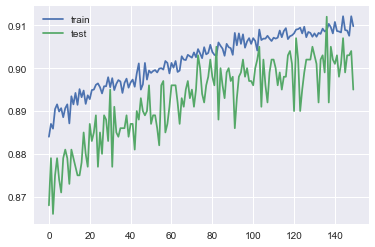
\includegraphics[height=0.4\textheight]{images/SUBJDataset_grad.png}
        			\caption{Precision of weight improving on SUBJ dataset for multiple epochs}
        		\end{figure}
        	\column{0.5\linewidth}

        		\begin{figure}[H]
        			\centering
        			\caption*{TFIDF + SVD + LR + gradient}
        			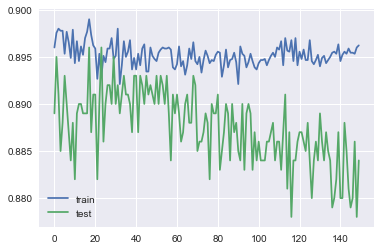
\includegraphics[height=0.4\textheight]{images/SUBJDataset_tfidf_grad.png}
        			\caption{Precision of tfidf weight improving on SUBJ dataset for multiple epochs}
        		\end{figure}
	\end{columns}        		
\end{frame} 



\begin{frame}{Plans}
    \begin{block}{}
        \begin{itemize}   
            \item Proper exploration of results
            \item Extend to bigrams
            \item Try transfer learning
            \item Try to extract the formula
            \item Try more complicated classifiers
            \item Try stochastic gradient \cite{brand2006fast}
        \end{itemize}
    \end{block}
\end{frame} 


\begin{frame}
    \vfill
    \begin{center}
        \huge\bfseries
        Thank you for your attention
        \vfill
    \end{center}
    \vfill
\end{frame}

\appendix

		\subsection{Literature}                
            \begin{frame}[allowframebreaks]{Literature}
			\footnotesize
				\nocite{*}
				\bibliographystyle{apalike}
				\bibliography{prezentacia.bib} 
            \end{frame}

\end{document}\grid
